\section{Resultados}

Através da matriz de confusão onde a fava cearense representa classes verdadeira, e a fava orelha de vó representada pela classe negativas, foi estriadas todas as métricas apresentada, duas delas é de grande importância como cobertura e precisão, isto é se o valor para a precisão fosse de 90\%, isto indicaria que a cada 100 mudas de fava classificadas como positivo, é esperado que apenas 90 seja de fava cearense. já a cobertura é razão entre a quantidade de exemplos classificados corretamente como positivos e a quantidade de exemplos que são de fato positivos, se o valor para a cobertura fosse de 95\%, isto indicaria que a cada 100 mudas de fava que são de fato positivos, é esperado que apenas 95 sejam corretamente identificados como fava uma das classes.  

\subsection{CNN}

Antes de utilizar o modelo como extrator de características, foi feito o treinamento de uma rede convolucional inteira. Ela é composta por duas camadas convolucionais, com filtros de tamanho 3×3 e 2x2, seguidas de camadas max pooling e dropout. Por fim, existem uma camadas totalmente conectadas e a camada de classificação mostrado na figura~\ref{fig:arquitetura_cnn}. Foi separada uma sub amostra de 30\% do conjunto de 1374 imagens totalizando 413 imagens, que foram utilizadas na validação dos modelos. Após isso, avaliação da rede convolucional, através da matriz de confusão notamos que das 413 acertou 182 da classe fava Cearense e 212 de fava Orelha de vó e teve instâncias teve 19 erros obtendo uma precisão de 0.94, com uma cobertura de 0.96 e a Área sob a curva AUC de 0.966.

% \begin{figure}[H]
% \centering
% \includegraphics[width=1.0\textwidth]{imagens/CNN_MLP.png}
% \caption{CNN MLP Resultados}
% \label{fig:cnn_mlp_result}
% \end{figure}

Na tabela~\ref{tabela:hiperparametros_best_models}, mostra os hiperparâmetros relacionado ao melhor modelo de CNN, obtidos através da seleção de modelos.

\begin{table}[H]
\centering
\caption{Hiper parâmetros dos Melhor Modelo CNN }
\label{tabela:hiperparametros_best_models}
\def\arraystretch{1.2}
\begin{tabular}{@{}lrrr@{}}
\toprule
{\textbf{Algoritimos}} & {\textbf{Hiperparâmetros}} & {\textbf{Variação}}  \\
\midrule
CNN MLP & epépocasochs & 364 \\ 
CNN MLP & tamanho do batch & 16\\ 
CNN MLP & otimizador & adam \\
CNN MLP & ativação & relu \\
CNN MLP & neurônios & 128 \\
CNN MLP & dropout & 0.1 \\
\bottomrule
\end{tabular}
\end{table}

\subsection{SVM}

Utilizando CNN com extrator de característica, removendo sua última camada a de classificação softmax. Assim, os valores de ativação dos neurônios da rede que estariam ligados nesta camada são utilizados como entrada à Maquina de Vetores de Suporte (SVM) para a classificação como mostra na figura~\ref{fig:esquematica_cnn}. Após isso, através da matriz de confusão, que das 413 instâncias acertou 197 da classe fava cearense e 201 de fava orelha de vó e teve 6 erros obtendo uma precisão de 0.98, com uma cobertura de 0.99 e a Área sob a curva AUC de 0.988.

%\begin{figure}[H]
%\centering
%\includegraphics[width=1.0\textwidth]{imagens/CNN_SVM.png}
%\caption{CNN SVM Resultados }
%\label{fig:svm_result}
%\end{figure}

Na tabela~\ref{tabela:hiperparametros_best_models}, mostra os hiperparâmetros relacionado ao modelo que obteve os melhores resultados, obtidos através da seleção de modelos.

\begin{table}[H]
\centering
\caption{Hiperparâmetros do Melhor Modelo SVM}
\label{tabela:hiperparametros_best_models_svm}
\def\arraystretch{1.2}
\begin{tabular}{@{}lrrr@{}}
\toprule
{\textbf{Algoritimos}} & {\textbf{Hiperparâmetros}} & {\textbf{Variação}}  \\
\midrule
CNN SVM & C & $2.91x10^{1}$ \\ %29.115026486768507 \\ 
CNN SVM & kernel & poly \\ 
CNN SVM & Grau do polinômio & 2 \\ 
CNN SVM & $\gamma$  & 
 $4.78x10^{-4}$ \\
% 0.0004780004165163952 \\
\bottomrule
\end{tabular}
\end{table}

Um dos fatores que levaram o SVM a se sobre sair são suas fronteiras otimizadas através do hipérmetro C que responsável por aplicando um custo durante o treinamento para cada amostra classificada erroneamente.

\subsection{Árvore de decisão}

Da mesma forma, Utilizando CNN com extrator de característica, removendo sua última camada a de classificação softmax. Assim, os valores de ativação dos neurônios da rede que estariam ligados nesta camada são utilizados na entrada de uma Árvore de Decisão para a classificação como mostra na figura~\ref{fig:esquematica_cnn}. Após isso, através da matriz de confusão, que das 413 instâncias acertou 186 da classe fava Cearense e 216 de fava Orelha de Vó e teve 11 erros obtendo uma precisão de 0.96, com uma cobertura de 0.98 e a Área sob a curva AUC de 0.979.

% \begin{figure}[H]
% \centering
% \includegraphics[width=1.0\textwidth]{imagens/CNN_TREE.png}
% \caption{CNN TREE Resultados }
% \label{fig:tree_result}
% \end{figure}

Na tabela~\ref{tabela:hiperparametros_best_models_tree}, mostra os hiperparâmetros relacionado ao modelo que obteve os melhores resultados, obtidos através da seleção de modelos.

\begin{table}[H]
\centering
\caption{Hiperparâmetros do Melhor Modelo Arvore}
\label{tabela:hiperparametros_best_models_tree}
\def\arraystretch{1.2}
\begin{tabular}{@{}lrrr@{}}
\toprule
{\textbf{Algoritimos}} & {\textbf{Hiperparâmetros}} & {\textbf{Variação}}  \\
\midrule
CNN TREE & criterion & gini \\ 
CNN TREE & max depth &   436 \\ 
CNN TREE & max leaf nodes & 861 \\ 
CNN TREE & min samples leaf & $9.17x10^{-2}$ \\ % 0.0917183949330819 \\  
CNN TREE & min samples split & $7.79x10^{-1}$ \\ %  0.7796910002727693 \\ 
CNN TREE & splitter & best \\ 
\bottomrule
\end{tabular}
\end{table}

\subsection{VGGNet}

Este experimento foi realizado de forma adicional, utilizando Transferência de Aprendizado (transfer learning) como arquitetura vgg16 treinados com os pesos da imagenet \cite{ImageNet}, com extrator de característica, removendo a camada totalmente conectada e substituindo por uma arquitetura de MLP, a mesma configuração utilizada nas camadas totalmente conectadas da CNN já descritas. Os Resultados obtido com está abordagem, através da matriz de confusão, que das 413 instâncias acertou 186 da classe fava cearense e 212 de fava Orelha de Vó e teve 15 erros obtendo uma precisão de 0.95, com uma cobertura de 0.96 e a Área sob a curva AUC de 0.974.

% \begin{figure}[H]
%  \centering
%     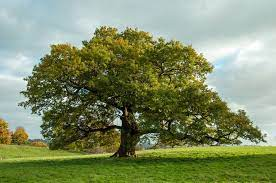
\includegraphics[width=1.0\textwidth]{imagens/transferir.png}
%     \caption{ CNN VGG16 Resultados }
%     \label{fig:vgg16_result}
% \end{figure}


Na tabela~\ref{tabela:hiperparametros_best_models_vgg}, mostra os hiperparâmetros relacionado ao modelo que obteve os melhores resultados, obtidos através da seleção de modelos.

\begin{table}[H]
\centering
\caption{Hiperparâmetros do Melhor Modelo Arvore}
\label{tabela:hiperparametros_best_models_vgg}
\def\arraystretch{1.2}
\begin{tabular}{@{}lrrr@{}}
\toprule
{\textbf{Algoritimos}} & {\textbf{Hiperparâmetros}} & {\textbf{Variação}}  \\
\midrule
VGG16 MLP & épocas & 166 \\ 
VGG16 MLP & tamanho do batch & 32\\ 
VGG16 MLP & otimizador & nadam \\
VGG16 MLP & ativação & relu \\
VGG16 MLP & neurônios & 64 \\
VGG16 MLP & dropout & 0.1 \\
\bottomrule
\end{tabular}
\end{table}

\label{sec:resultados}